%% wlkr
\documentclass[12pt,journal,compsoc]{IEEEtran}
\usepackage{graphicx}

\begin{document}
\title{Using Twitter Data and Sentiment Analysis to Predict Future Values of Cryprocurrencies}

\author{Ryan Walker}

\IEEEtitleabstractindextext{%
\begin{abstract}
This paper presents numerical schemes for gathering, processing and correlating sentiment data to actual cost 
for a given crypocurrency over a given unit of time in the interest in finding a time-lagged correlation. 
\end{abstract}
}

% make the title area
\maketitle
\IEEEpeerreviewmaketitle

\section{Introduction}
\IEEEPARstart{S}{entiment} analysis techniques have been used for stock market predictions in the past  with 
mixed success \cite{BI1}. We are of the opinion that for a technique like this to work there are three major requirements.

\begin{enumerate}
\item High volume of sentiment source;
\item Strong correlation to trader action and community opinion, and
\item Low quantity of non-deterministic value changing artifacts: news reports, earnings, company announcements, etc.
\end{enumerate}

In most cases, points one and three are mutually exclusive, meaning if there is a high volume of people talking about a
stock publicly $\frac{100k+}{Day}$, the company will typically be publishing earning reports, posting news, etc... 
These are important for investors, but cannot be accurately modeled as they are considered random artifacts.\\

As there are still news artifacts regarding Cryptocurrencies, they are less common and typically 
have less of an impact because unless there is a major problem with the algorithm, they are mostly subjective, unlike 
an earning report or other financial documents.\\

The aim of this paper is to attempt to validate what has been listed above, and use the data to make further informed 
buys and sells.

\subsection{Gathering Sentiment Data}
The main source of sentiment data was from twitter. The Python module \textit{tweepy} \cite{Tweepy} was used to gather
tweets and bin them into cryptocurrencies of interest. The volume was anywhere from $1.2k \frac{tweets}{hr}$
to $24k \frac{tweets}{hr}$ depending on the currency of interest. For this paper we were mostly interest in BTC, as the
tweet volume is the highest; in the past five months, we have gathered over 21 billion tweets on Bitcoin alone.\\

Once the data is gathered it is put into a time series dataset with a period of 30 seconds - from that point Python \textit{NLTK} 
(Natural Language Toolkit) \cite{NLTK} is used to perform sentiment analysis to rate each tweet and make a net sum per unit time,
as shown in Figure \ref{fig:RawSent}. 

\begin{figure}[hp]
	\centering
	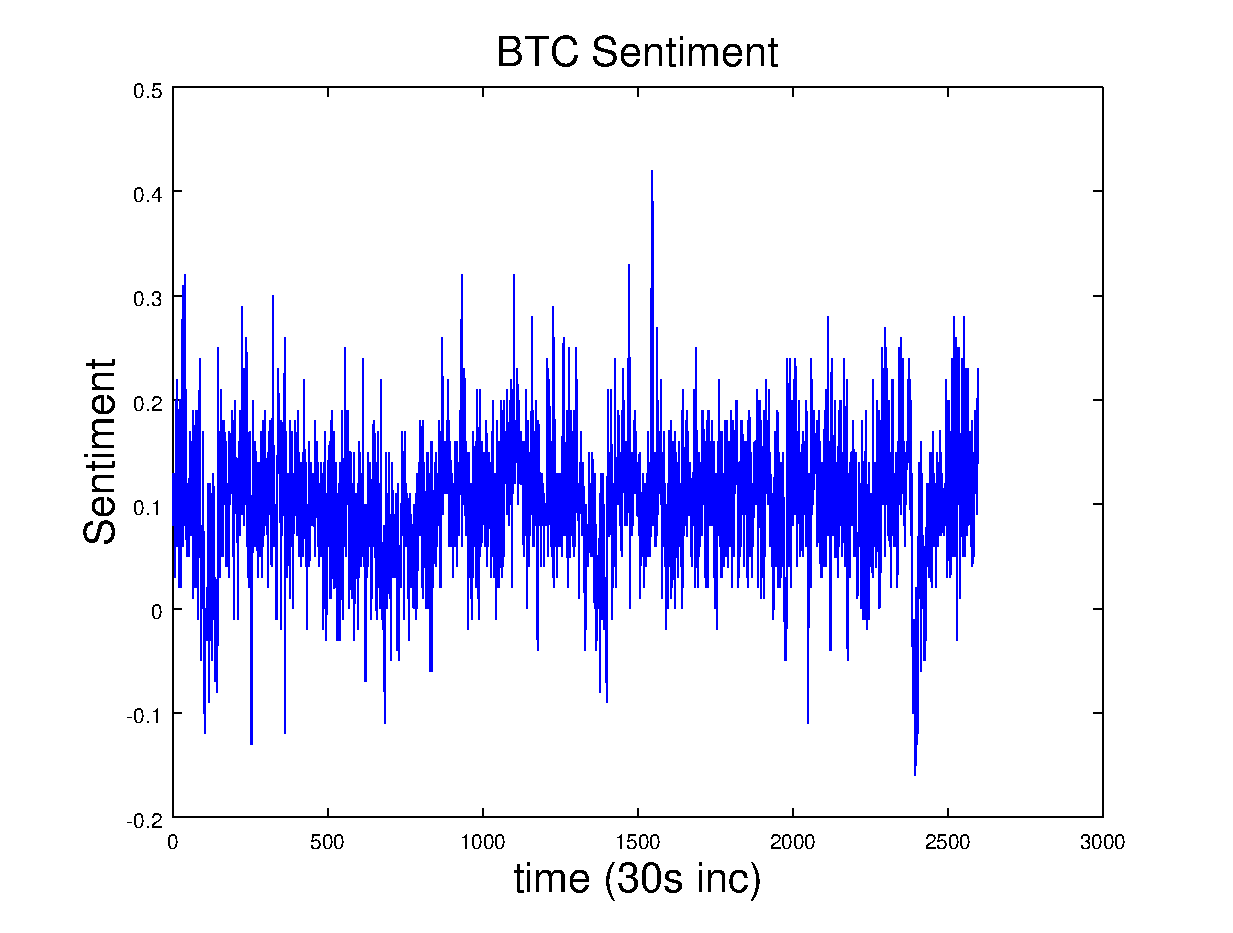
\includegraphics[width=0.5\textwidth]{../Datasets/Plots/Oct9_Sen}
	\caption{Raw Sentiment, October 9th 2017}
	\label{fig:RawSent}
\end{figure}

The filtered signal is shown in Figure \ref{fig:FilteredSent} - it's possible to compare the sentiment and values time series.

\begin{figure}[h]
	\centering
	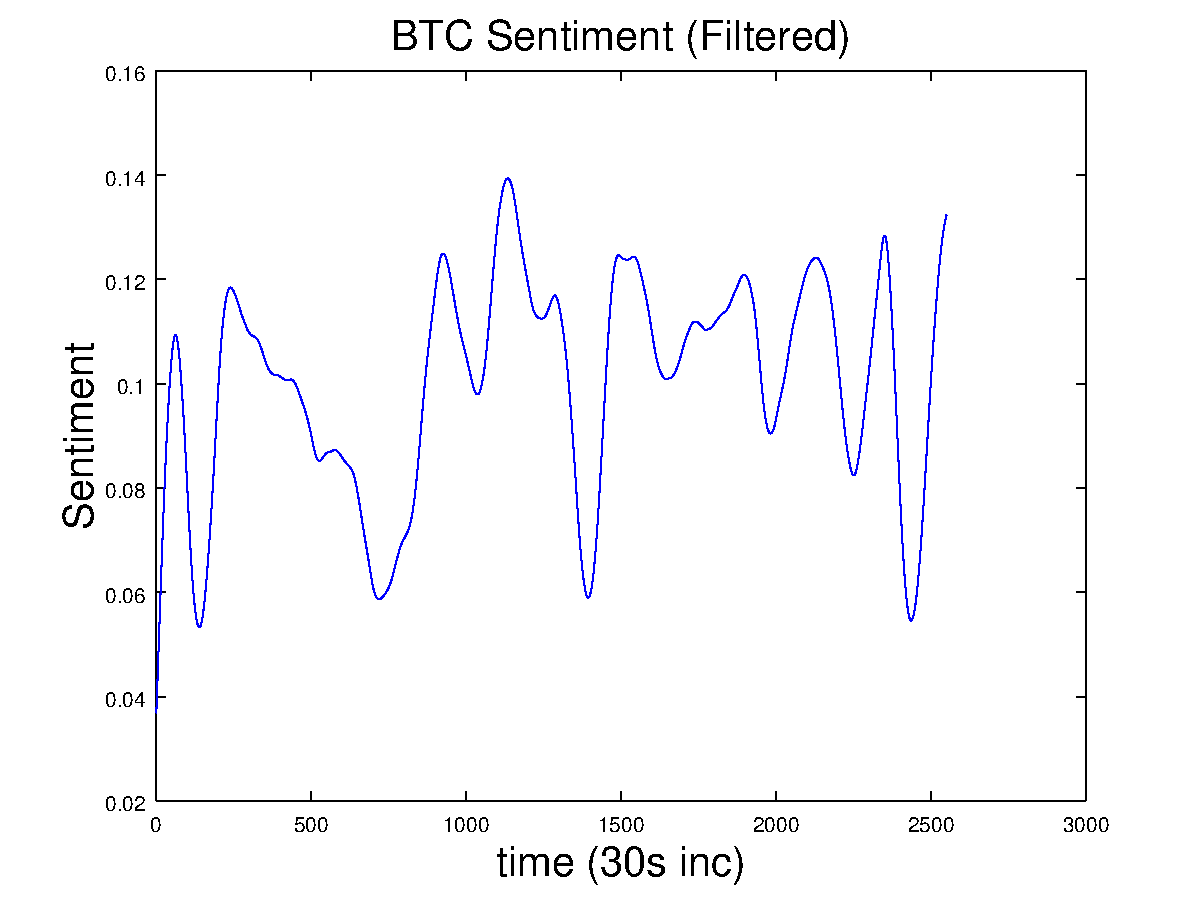
\includegraphics[width=0.5\textwidth]{../Datasets/Plots/Oct9_Sen_Fil}
	\caption{Filtered Sentiment, October 9th 2017}
	\label{fig:FilteredSent}
\end{figure}

\subsection{Timewise Correlation}
The timewise correlation was calculated using the correlation vector $k$,

\begin{equation}\label{eq:K}
k_j = \frac{\sum\limits_{i=0}^n \dot{x}_i - \dot{y}_{i+j}}{n-j},\quad j=0,\dots,n
\end{equation}

\noindent where $x$ denotes the cost of the currency and $y$ the sentiment.\\ 

The reasoning for using derivatives 
for the correlation is simply because the sentiment values are effectively a floating quantity -- 
the magnitude of the sentiment is not believed to have any direct relationship with the magnitude of the cost.
In other words we are looking for a correlation between the change in sentiment with the change in cost. 
This is justified by the success of our analysis\\

\begin{figure}[h]
	\centering
	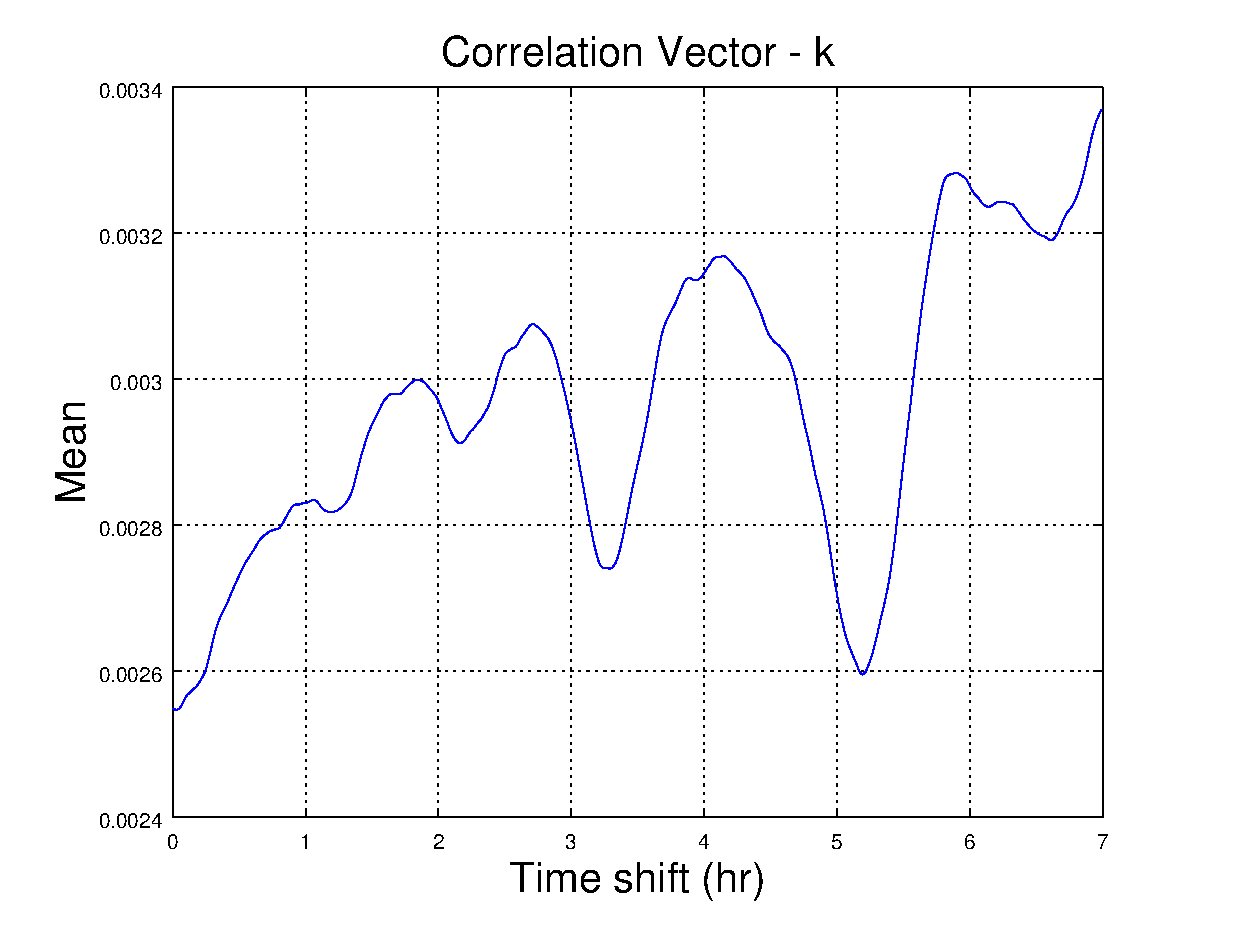
\includegraphics[width=0.5\textwidth]{../Datasets/Plots/Oct7_K}
	\caption{Time Correlation vector $k$, October 7th 2017}
	\label{fig:K}
\end{figure}

We look for local minima in of $k$ as these points indicate the highest level of signal similarity.
As seen in Figure \ref{fig:K}, $k$ has a global minima around 5.2hrs, which is defined as $\tau_L = 5.2hrs$ 
or the effective time lag between high values of changing sentiment and high values of changing cost.\\

We observe that the calculation of $\tau_L$ has been repeatable over a given unit of time. Figure \ref{fig:Ksum} 
shows the vector sum of 15 $k$ vectors from November 2nd to November 17th. In addition there are some interesting 
patterns appearing as local minima at $\sim1.8hrs$ and $\sim3.2hrs$.

\begin{figure}[h]
	\centering
	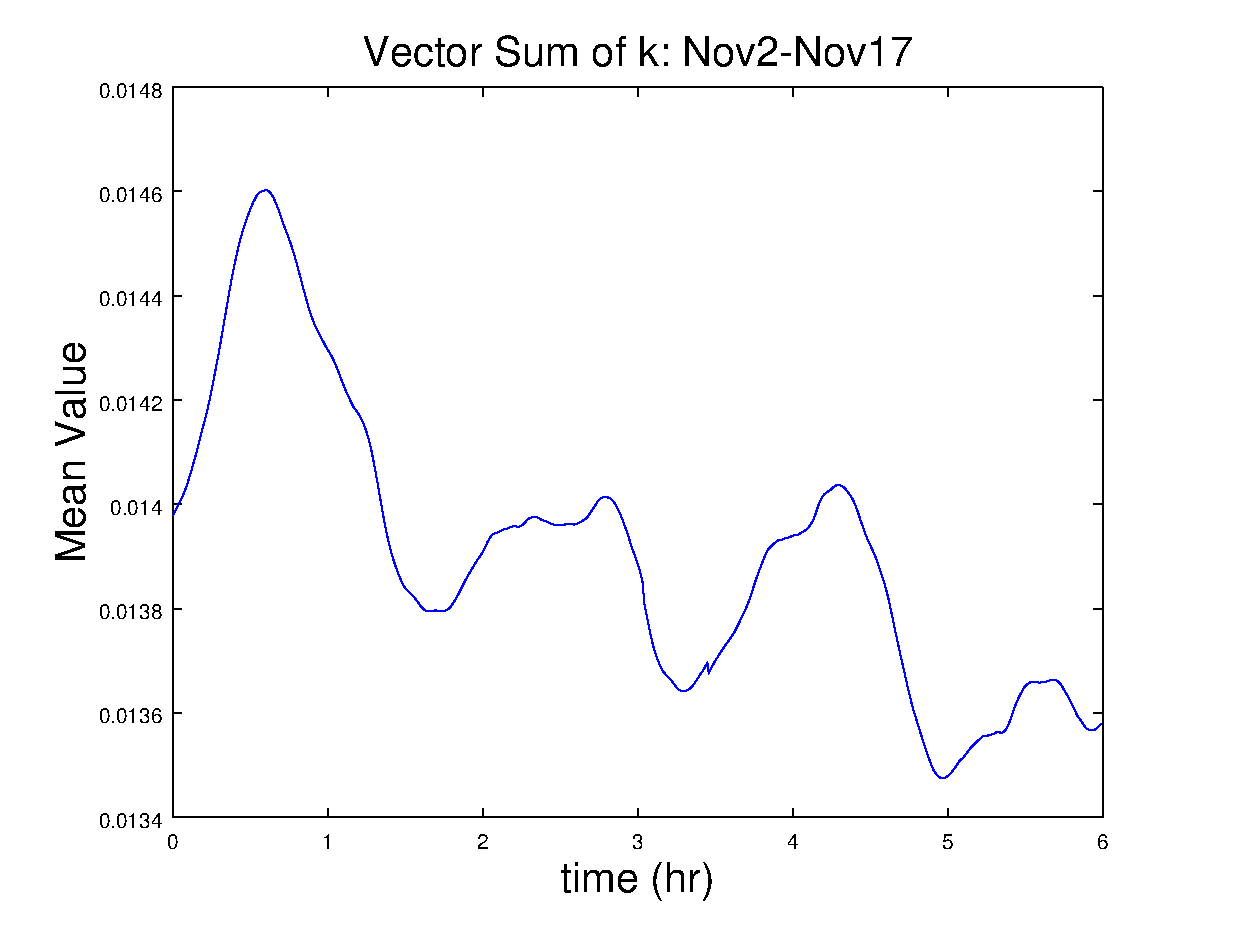
\includegraphics[width=0.5\textwidth]{../Datasets/Plots/VectorSumk}
	\caption{Mean Time Correlation vector $k$, Nov2 - Nov17, 2017}
	\label{fig:Ksum}
\end{figure}

Figure \ref{fig:SentShift} shows the sentiment shifted forward in time by $\tau_L$. The 
rates of high change and local minima and maxima are matched between the two datasets, see also
figures \ref{fig:Dec23} to \ref{fig:Dec4-8}. 

\begin{figure}[h]
	\centering
	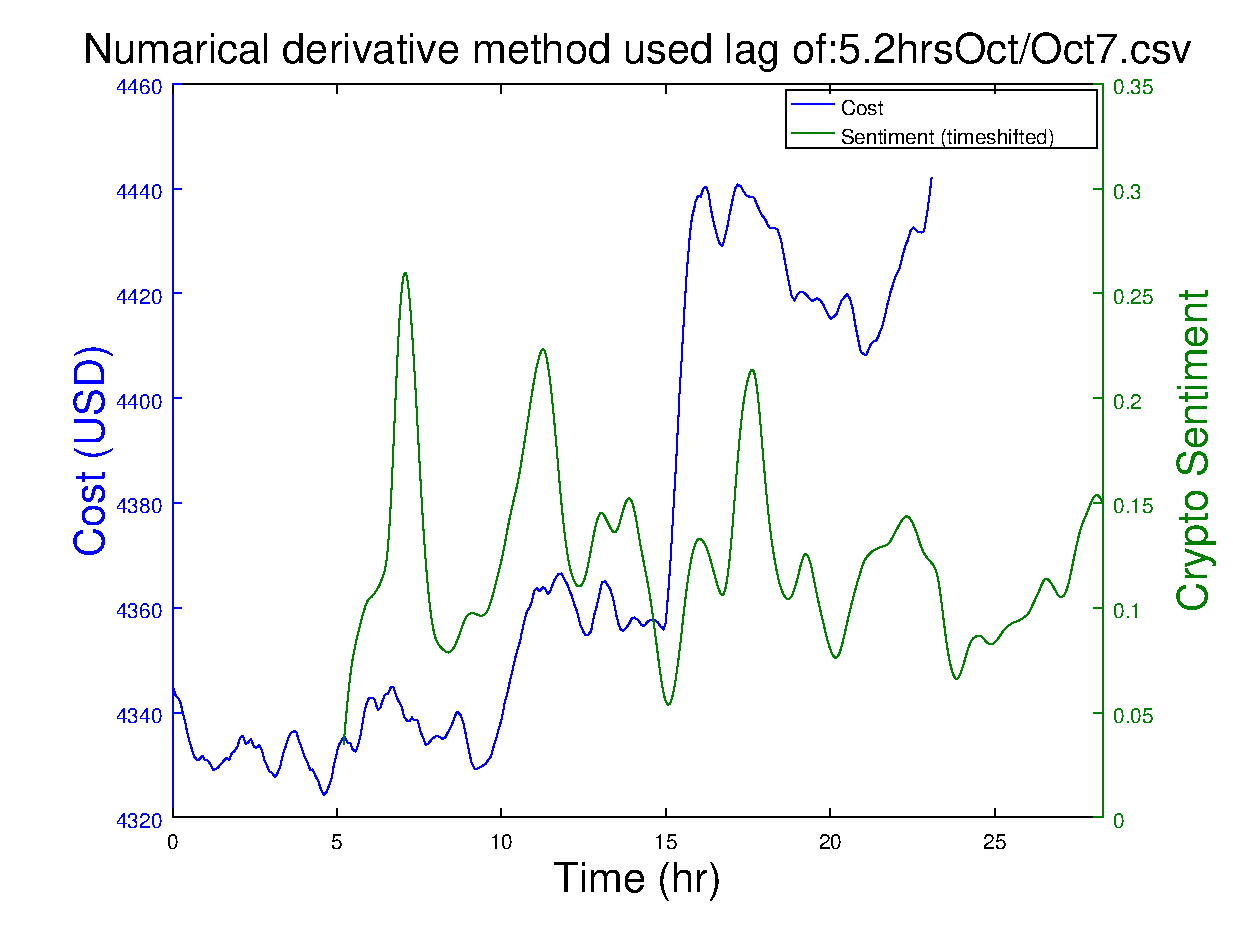
\includegraphics[width=0.5\textwidth]{../Datasets/Plots/Oct7_CostSen}
	\caption{Time Shifted Sentiment, October 9th 2017}
	\label{fig:SentShift}
\end{figure}

\subsection{Realtime Implementation}
Moving into a real time implementation was simple enough; previously the data post processing was being done in Octave, for the 
real time implementation Python was used. The application followed this structure,
\begin{enumerate}
	\item $\tau = 10hrs$ of data is gathered.
	\item Data is filtered, $k$ and hence $\tau_L$ are calculated.
	\item Buy and sell triggers are found, using the data from $\tau - \tau_L$, where $\tau$ is the current time.
	\item Finally, Push notifications are sent to a mobile device using pushover \cite{Pushover}.
\end{enumerate}
%rework
The crux of the realtime application is finding the trigger points. 
happen in $\tau_L$ time. 
%rework
Is is expected that current high values of $\dot{y}$ correlate to high values of $\dot{x}$ in time $\tau_L$.
So high slope positive and negative values were taken and
labeled as buy and sell triggers respectively. This is one possible method of finding the triggers, but further work
should be done to understand if this is the best.

This realtime application is currently running and sending out advice for HFT (high frequency trading).
\section{Future work} %Move this into conclusion
\subsection{Optimisation problem}
The parameters in the real time application that are in need of optimisation. 
\begin{itemize}
	\item $\tau$ - the amount of data to collect in the real time app before starting the post operations.
	\item Number of buy/sell triggers, per $\tau$.
	\item Stronger understanding of the Time Zone Inference (See appendix).
	\item Threshold for buy/sell triggers, what counts a 'high sentiment'.
	\item Filter cutoff frequency.
\end{itemize}
We could optimize each parameter using our existing dataset.
This would be extremely computational expensive most likely require offloading to an HPC environment.

\subsection{Machine Learning}
It's possible that there are correlations in the dataset that are not distinguishable by humans. Treating the problem
like a black box and using a deep neural net it might be possible to gain a deeper understanding of trends and better results. 
In addition, we believe we could also use Bayesian inference techniques.

\subsection{Public Accessibility}
All the work that has been done could be rolled into a pay to access platform to which users can subscribe to make informed
trading decisions.

\section{Conclusion} %Roll future work into this. Just because the conclusion sucks balls
The crypto currency landscape is rapidly changing, as newly opened exchanges have facilitated access in the investment of 
decentralised currencies. 
%Rework
This gives reason to believe that in addition to understanding 
the tech, it's also interesting to understand what people are thinking about the tech. 
%Rework
This is important because the majority 
vote will determine the most widely adopted currency.\\

This was partially demonstrated in the work done above, but there's much more work that can be done. Analysis of other platforms
other than just Twitter we believe it's possible to see an even better results. Aggregating a larger dataset could be 
used to understand the limitations of currencies and how volume spikes affect their network.

\section{Appendix}
\subsection{Time Zone Inferance}
There are also highly observable daily oscillations in tweet volume as seen in Figure \ref{fig:OSC}. 
These can be used to infer time zones of maximum influence.
\begin{figure}[h!]
	\centering
	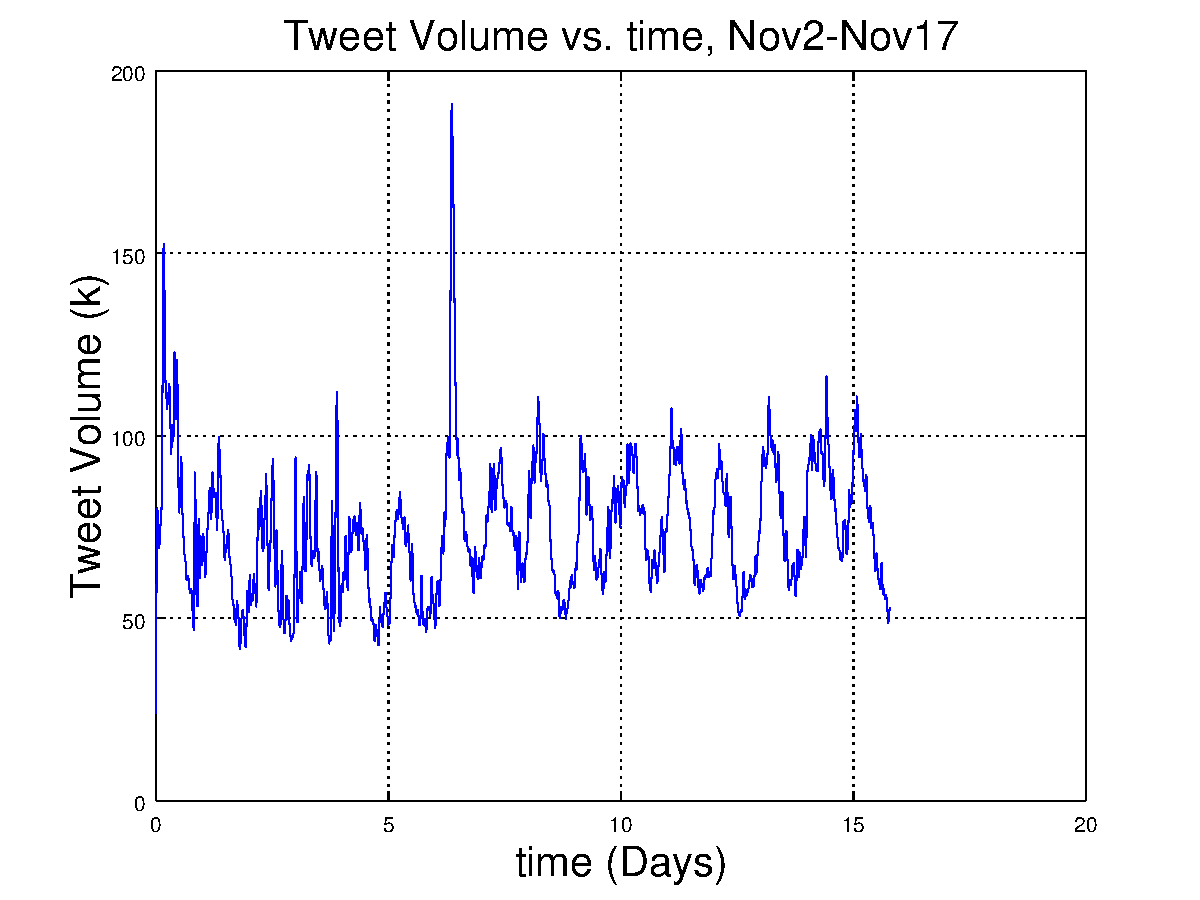
\includegraphics[width=0.5\textwidth]{../Datasets/Plots/TweetVolume}
	\caption{Tweet volume, Nov2 - Nov17, 2017}
	\label{fig:OSC}
\end{figure}

\subsection{Additional Data}

\begin{figure}[h!]
	\centering
	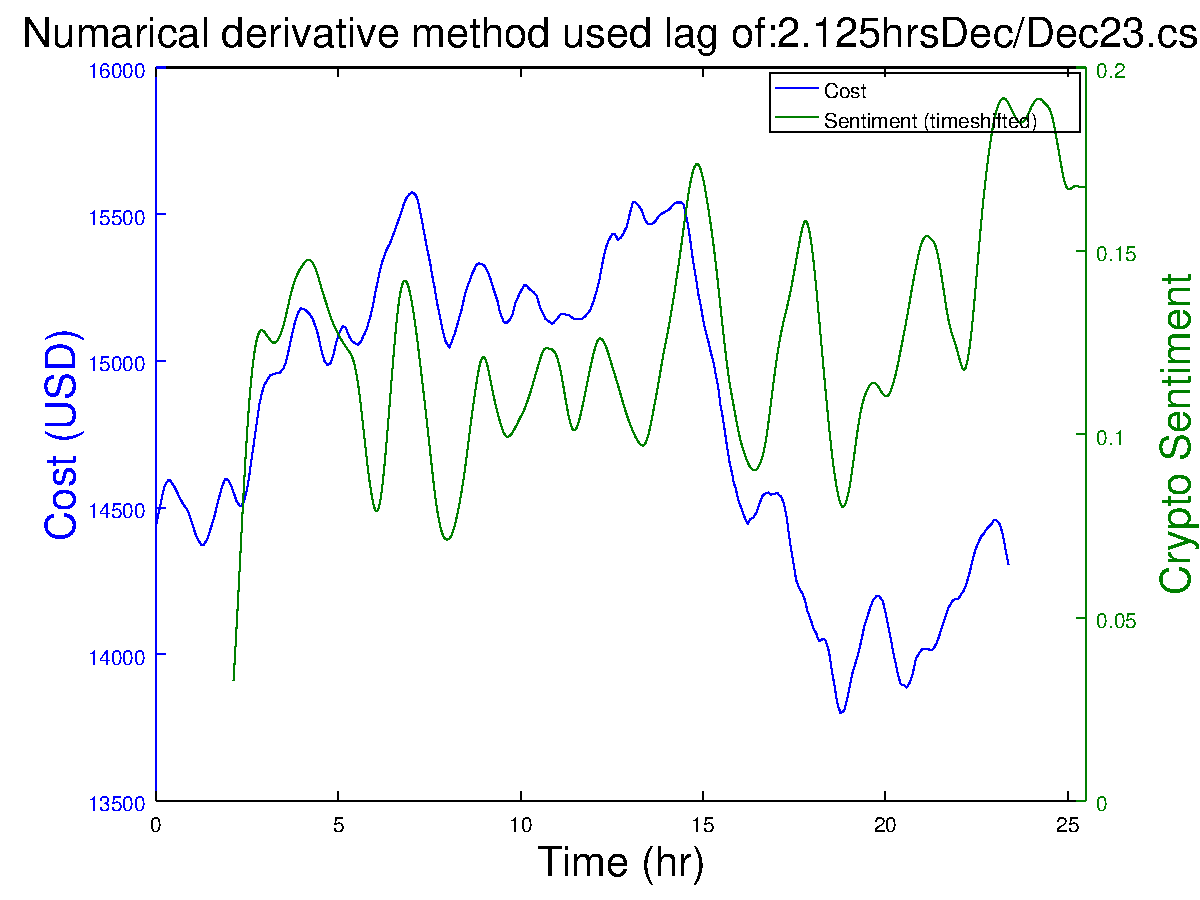
\includegraphics[width=0.5\textwidth]{../Datasets/Plots/Dec23}
	\caption{Dec23}
	\label{fig:Dec23}
\end{figure}

\begin{figure}[h!]
	\centering
	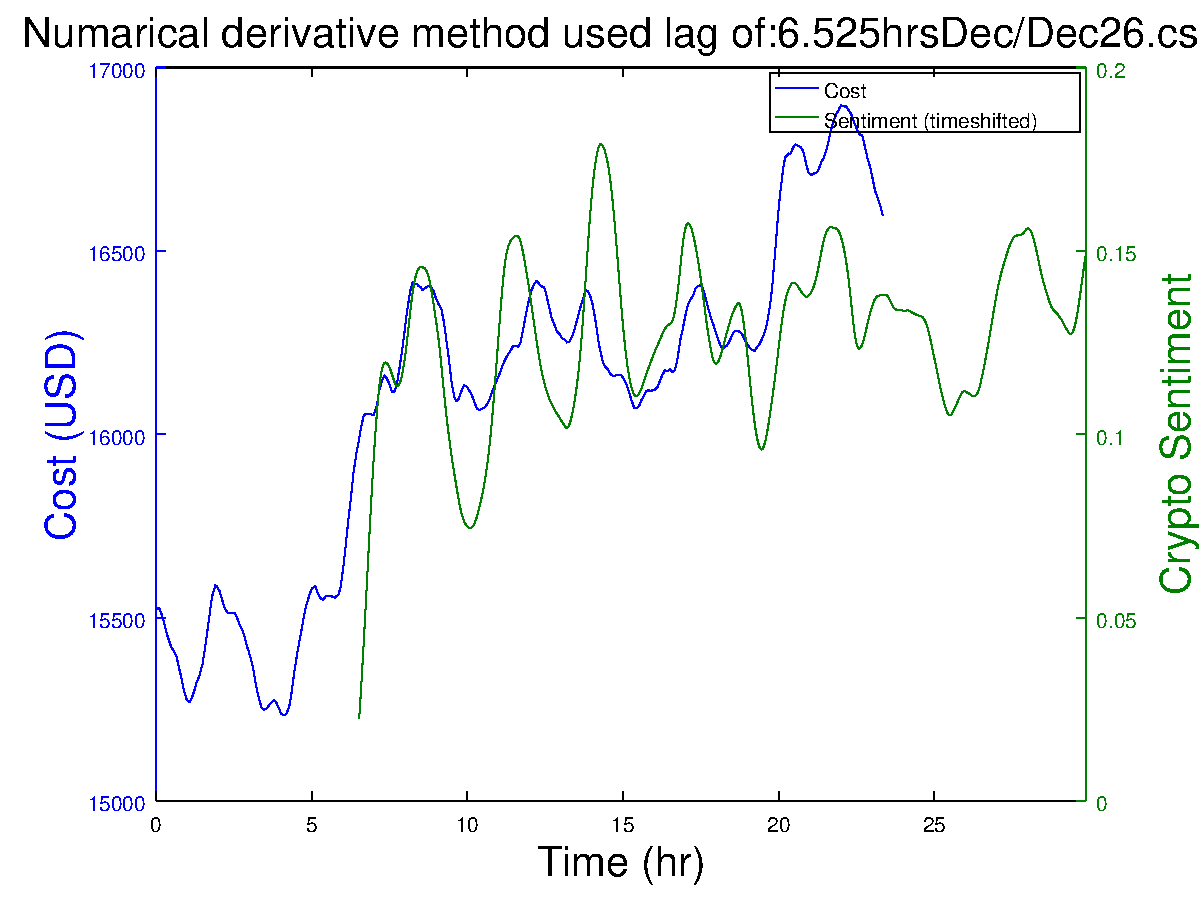
\includegraphics[width=0.5\textwidth]{../Datasets/Plots/Dec26}
	\caption{Dec26}
	\label{fig:Dec26}
\end{figure}

\begin{figure*}[h!]
	\centering
	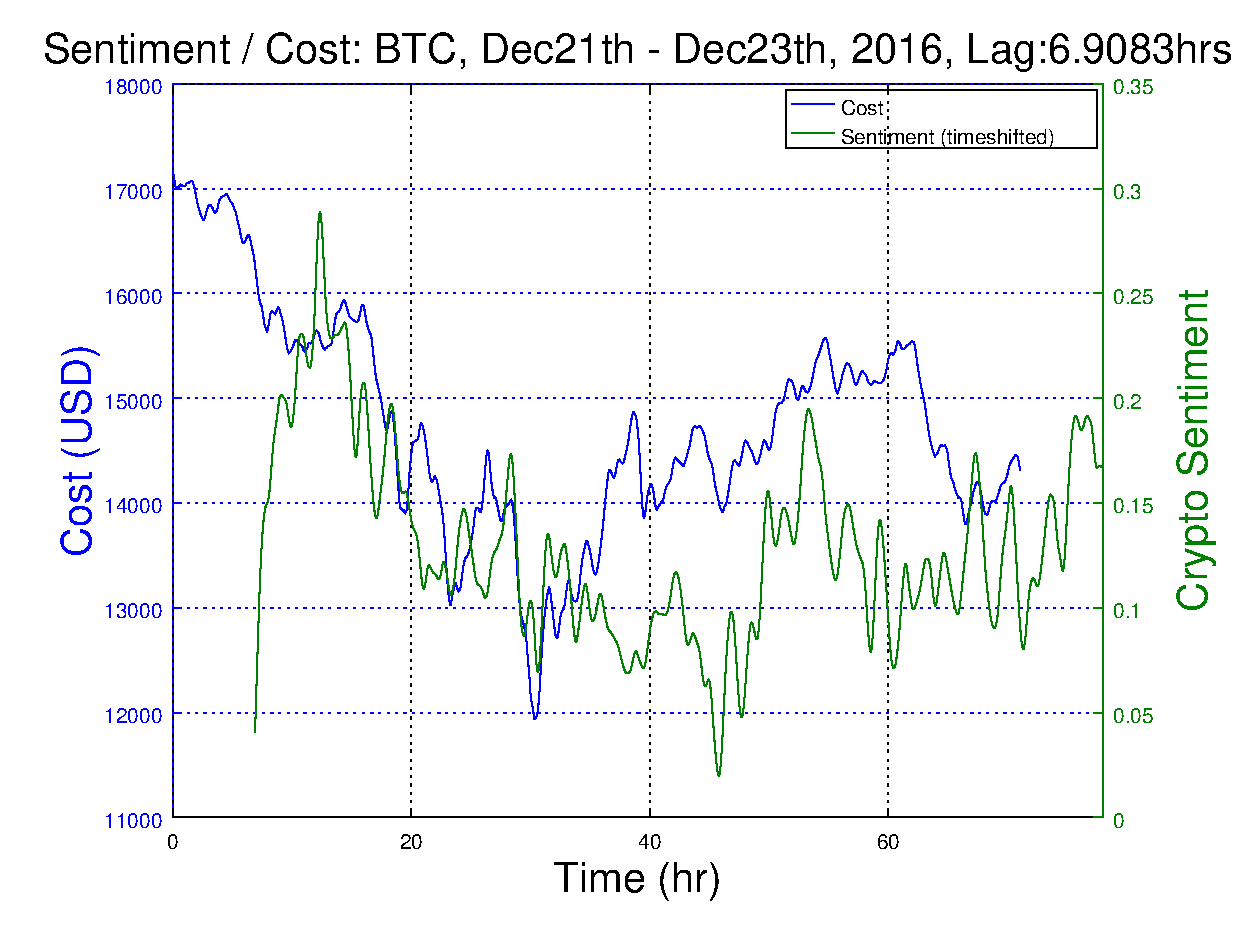
\includegraphics[width=0.8\textwidth]{../Datasets/Plots/Dec21-23}
	\caption{Bitcoin 'crash', Dec21 - Dec23, 2017}
	\label{fig:Dec21-23}
\end{figure*}

\begin{figure*}[h!]
	\centering
	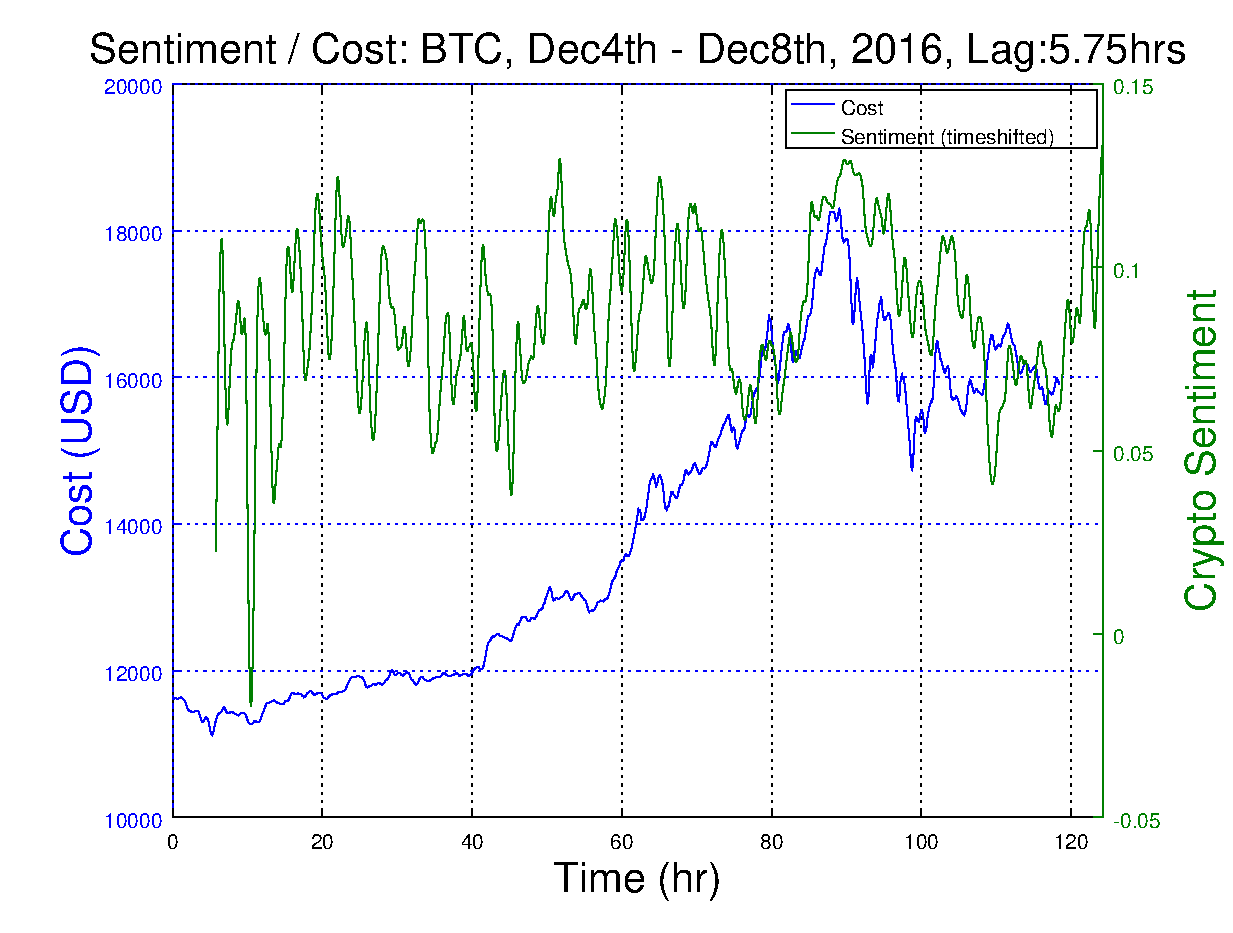
\includegraphics[width=0.8\textwidth]{../Datasets/Plots/Dec4-8}
	\caption{Four day trend - Dec4 - Dec8, 2017}
	\label{fig:Dec4-8}
\end{figure*}

\begin{thebibliography}{1}

\bibitem{BI1}
Anshul Mitta and Arpit Goel, \textit{Stock Prediction Using Twitter Sentiment Analysis}

\bibitem{Tweepy}
https://github.com/tweepy/tweepy

\bibitem{NLTK}
http://www.nltk.org/

\bibitem{Octave}
https://www.gnu.org/software/octave/

\bibitem{Pushover}
https://pushover.net/

\end{thebibliography}

\end{document}
